\begin{figure}
\centering
\begin{tabular}{ccc}
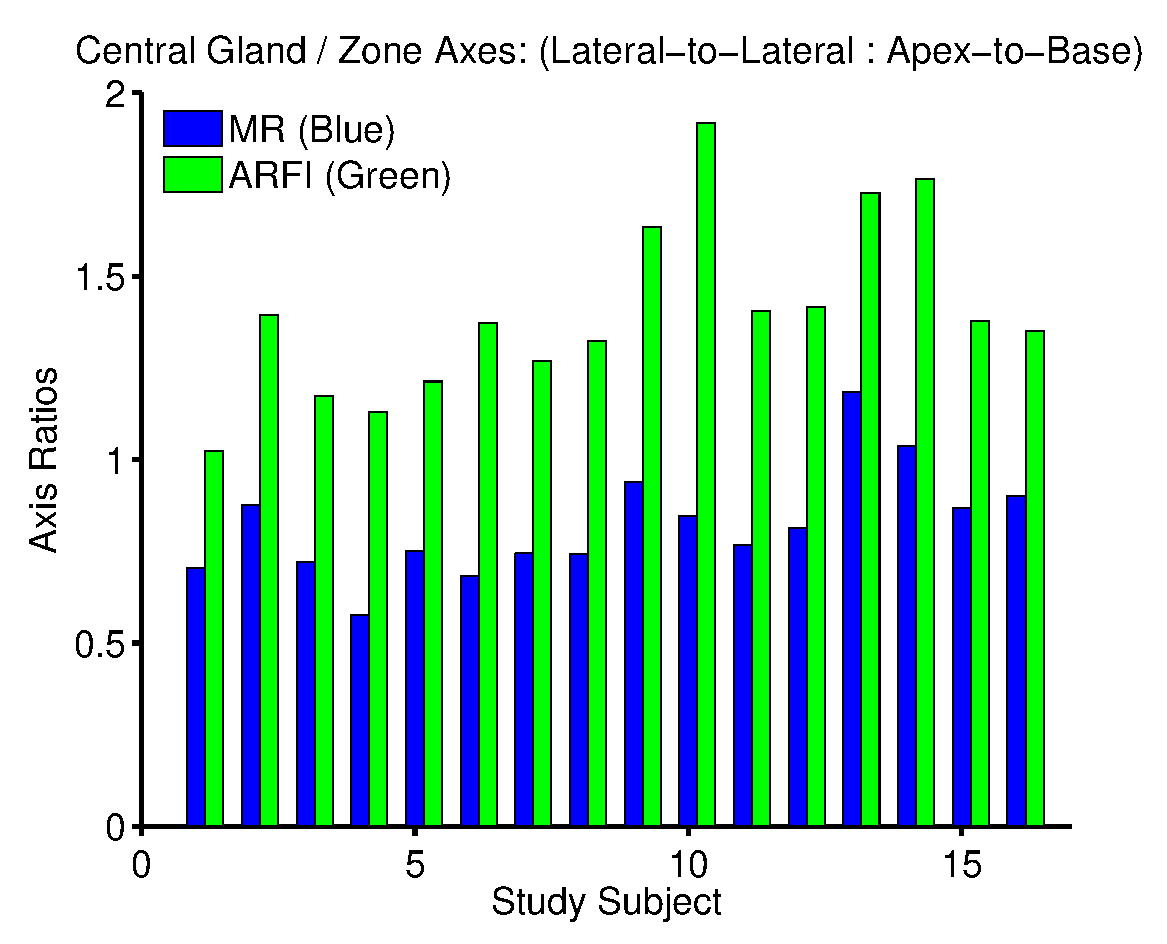
\includegraphics[width=0.3\linewidth]{figs/mr_arfi_central_axes1} &
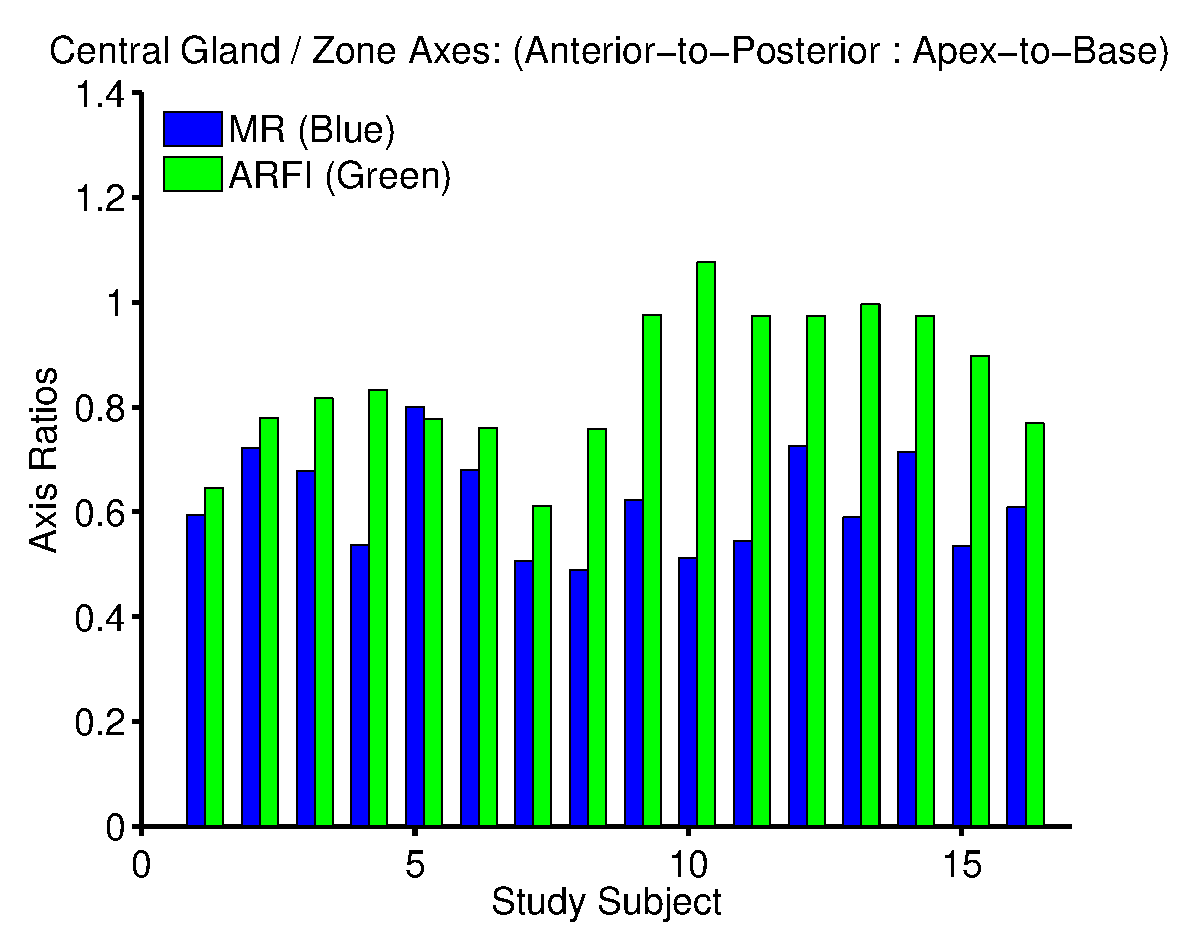
\includegraphics[width=0.3\linewidth]{figs/mr_arfi_central_axes2} &
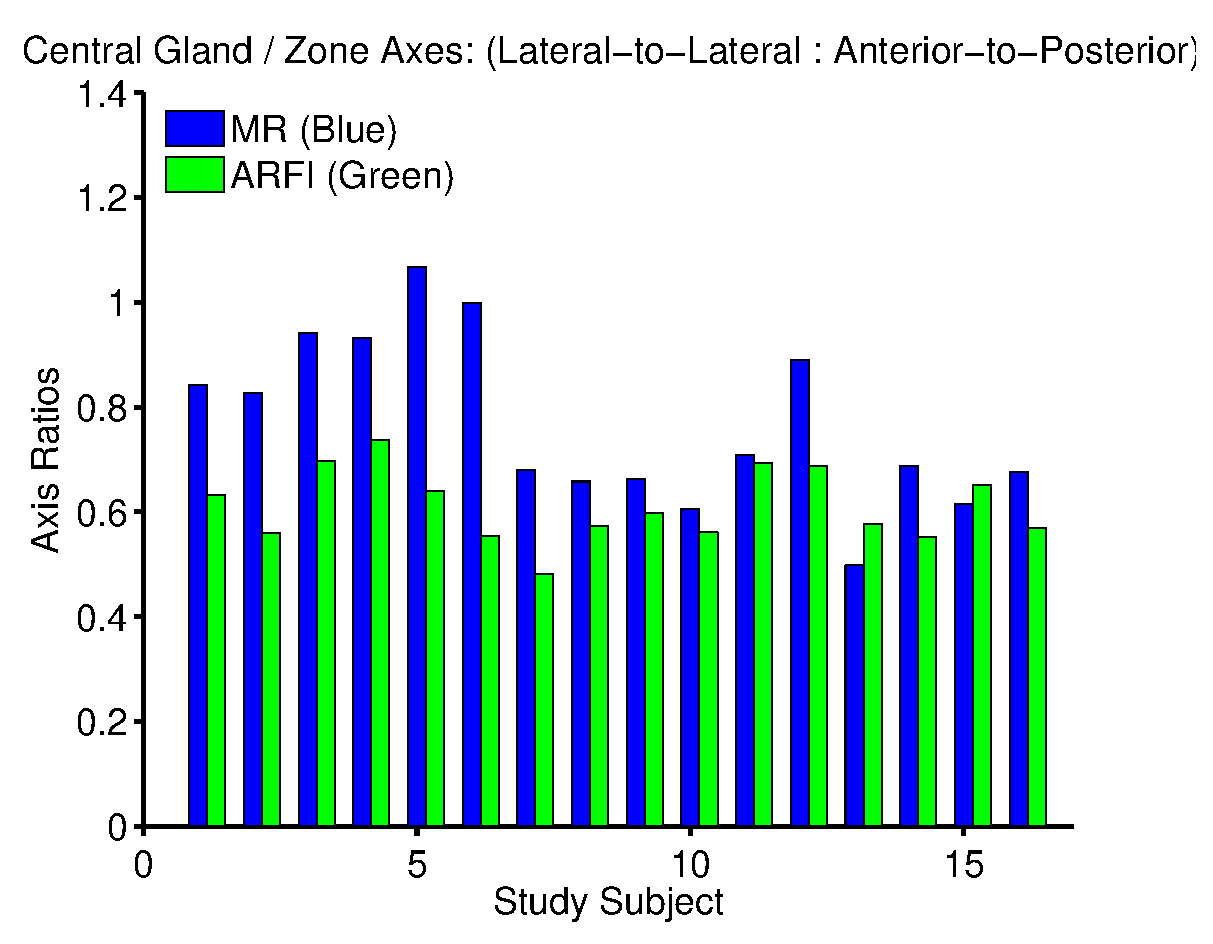
\includegraphics[width=0.3\linewidth]{figs/mr_arfi_central_axes3} \\
(a) & (b) & (c) \\
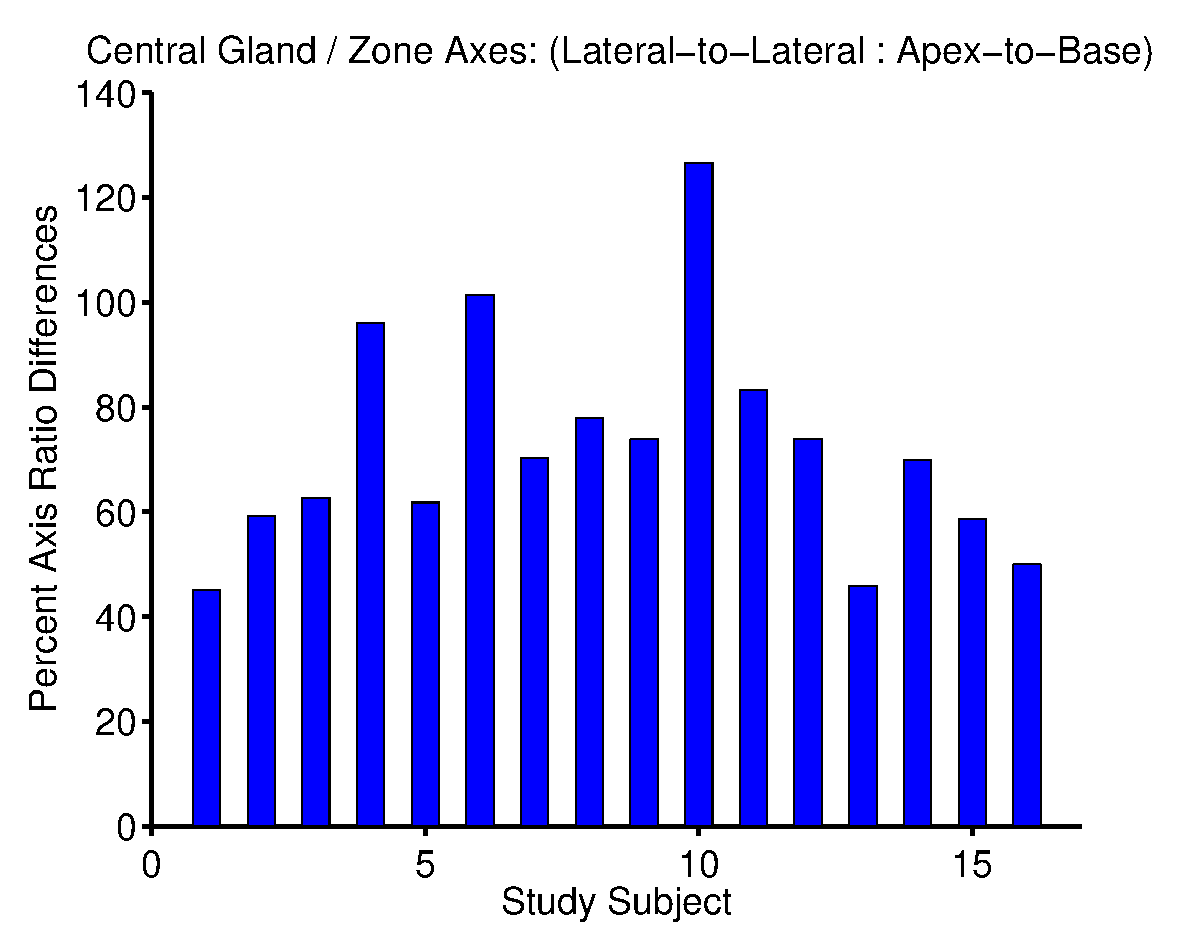
\includegraphics[width=0.3\linewidth]{figs/mr_arfi_central_over_under1.eps} &
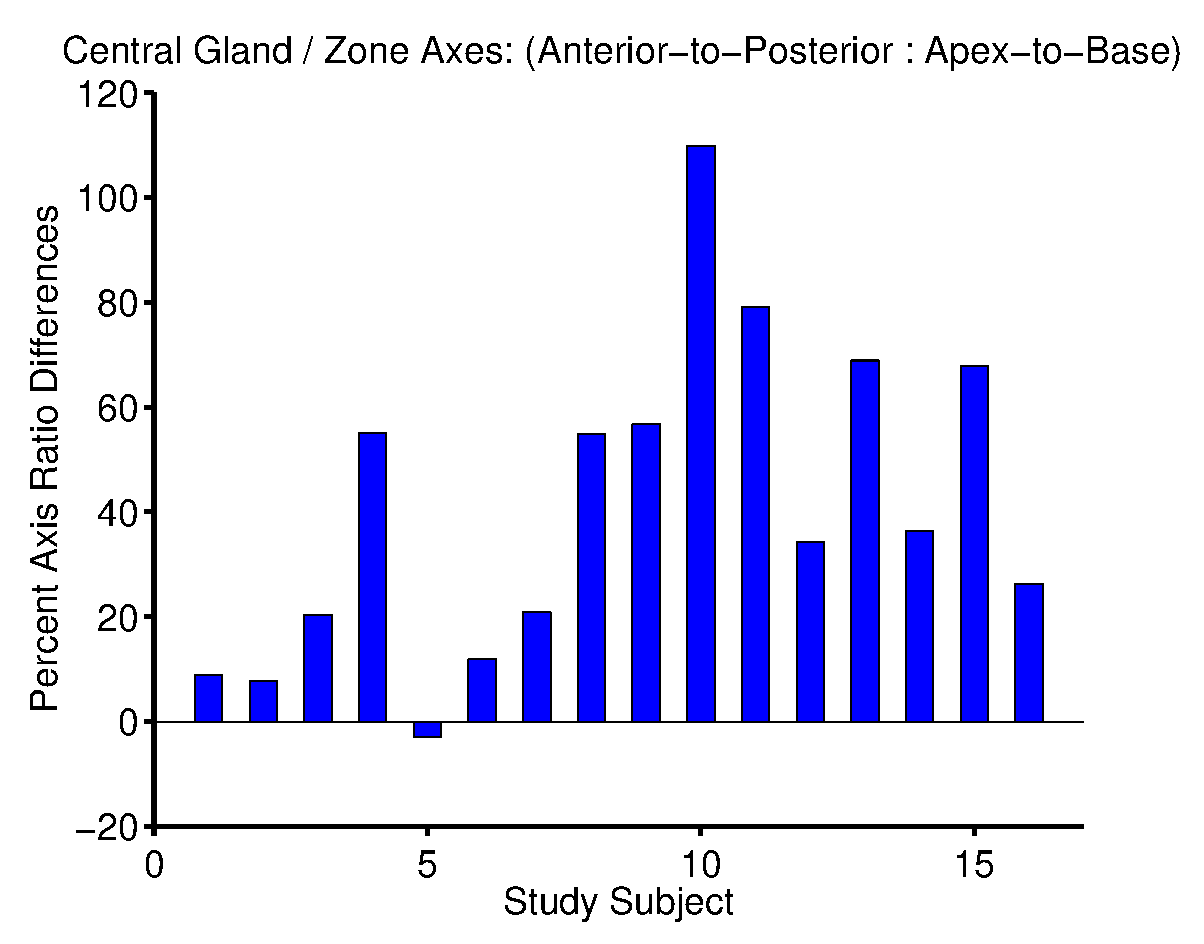
\includegraphics[width=0.3\linewidth]{figs/mr_arfi_central_over_under2.eps} &
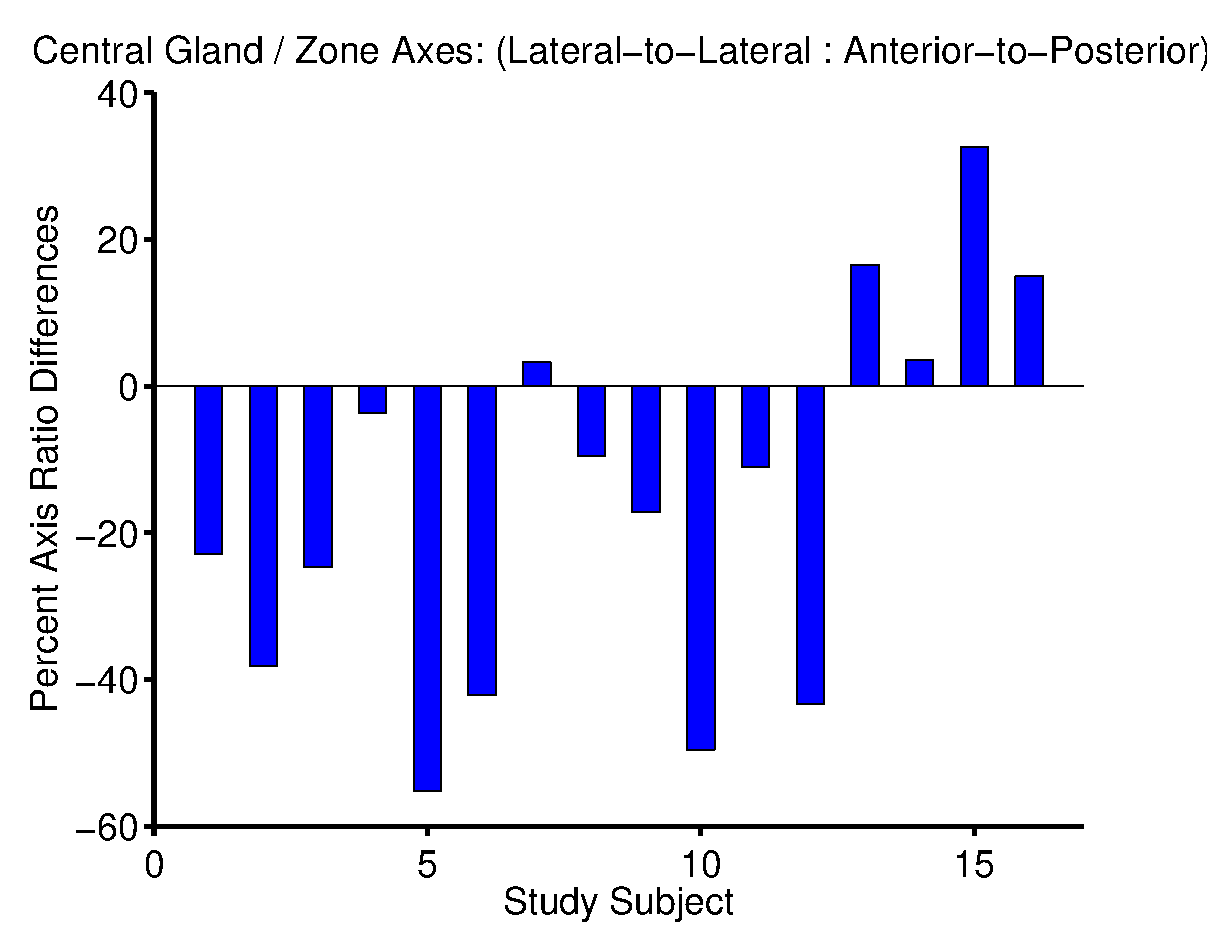
\includegraphics[width=0.3\linewidth]{figs/mr_arfi_central_over_under3.eps} \\
(a) & (b) & (c) \\
\end{tabular}
\caption{Comparison of the ratios of the three anatomic axis measurement ratios
    for T2WI MR (top row, blue) and ARFI imaging (top row, green).  The
    over/underestimation of the axis ratios between ARFI imaging and T2WI MR
    are shown in the bottom row (d-f), with mean ratio differences compiled in
    Table~\ref{tab:axis_ratio_over_under}.}
\label{fig:mr_arfi_central_axes} 
\end{figure}
